
\subsection{Resumen de objetivos}


\normalfont

El trabajo práctico consiste en el análisis del circuito de un amplificador de audio clase B, en la clásica configuración de 3 etapas, una entrada diferencial, una etapa VAS y una etapa de salida clase B.


\subsection{Desarrollo}

El análisis pedido consiste en llevar el circuito a un punto Q determinado para luego hacer un análisis de su THD en diferentes condiciones. En la figura~\figref{fig:fig_original_circuit} se observa el circuito propuesto.


\begin{figure}[H] %htb
\begin{center}
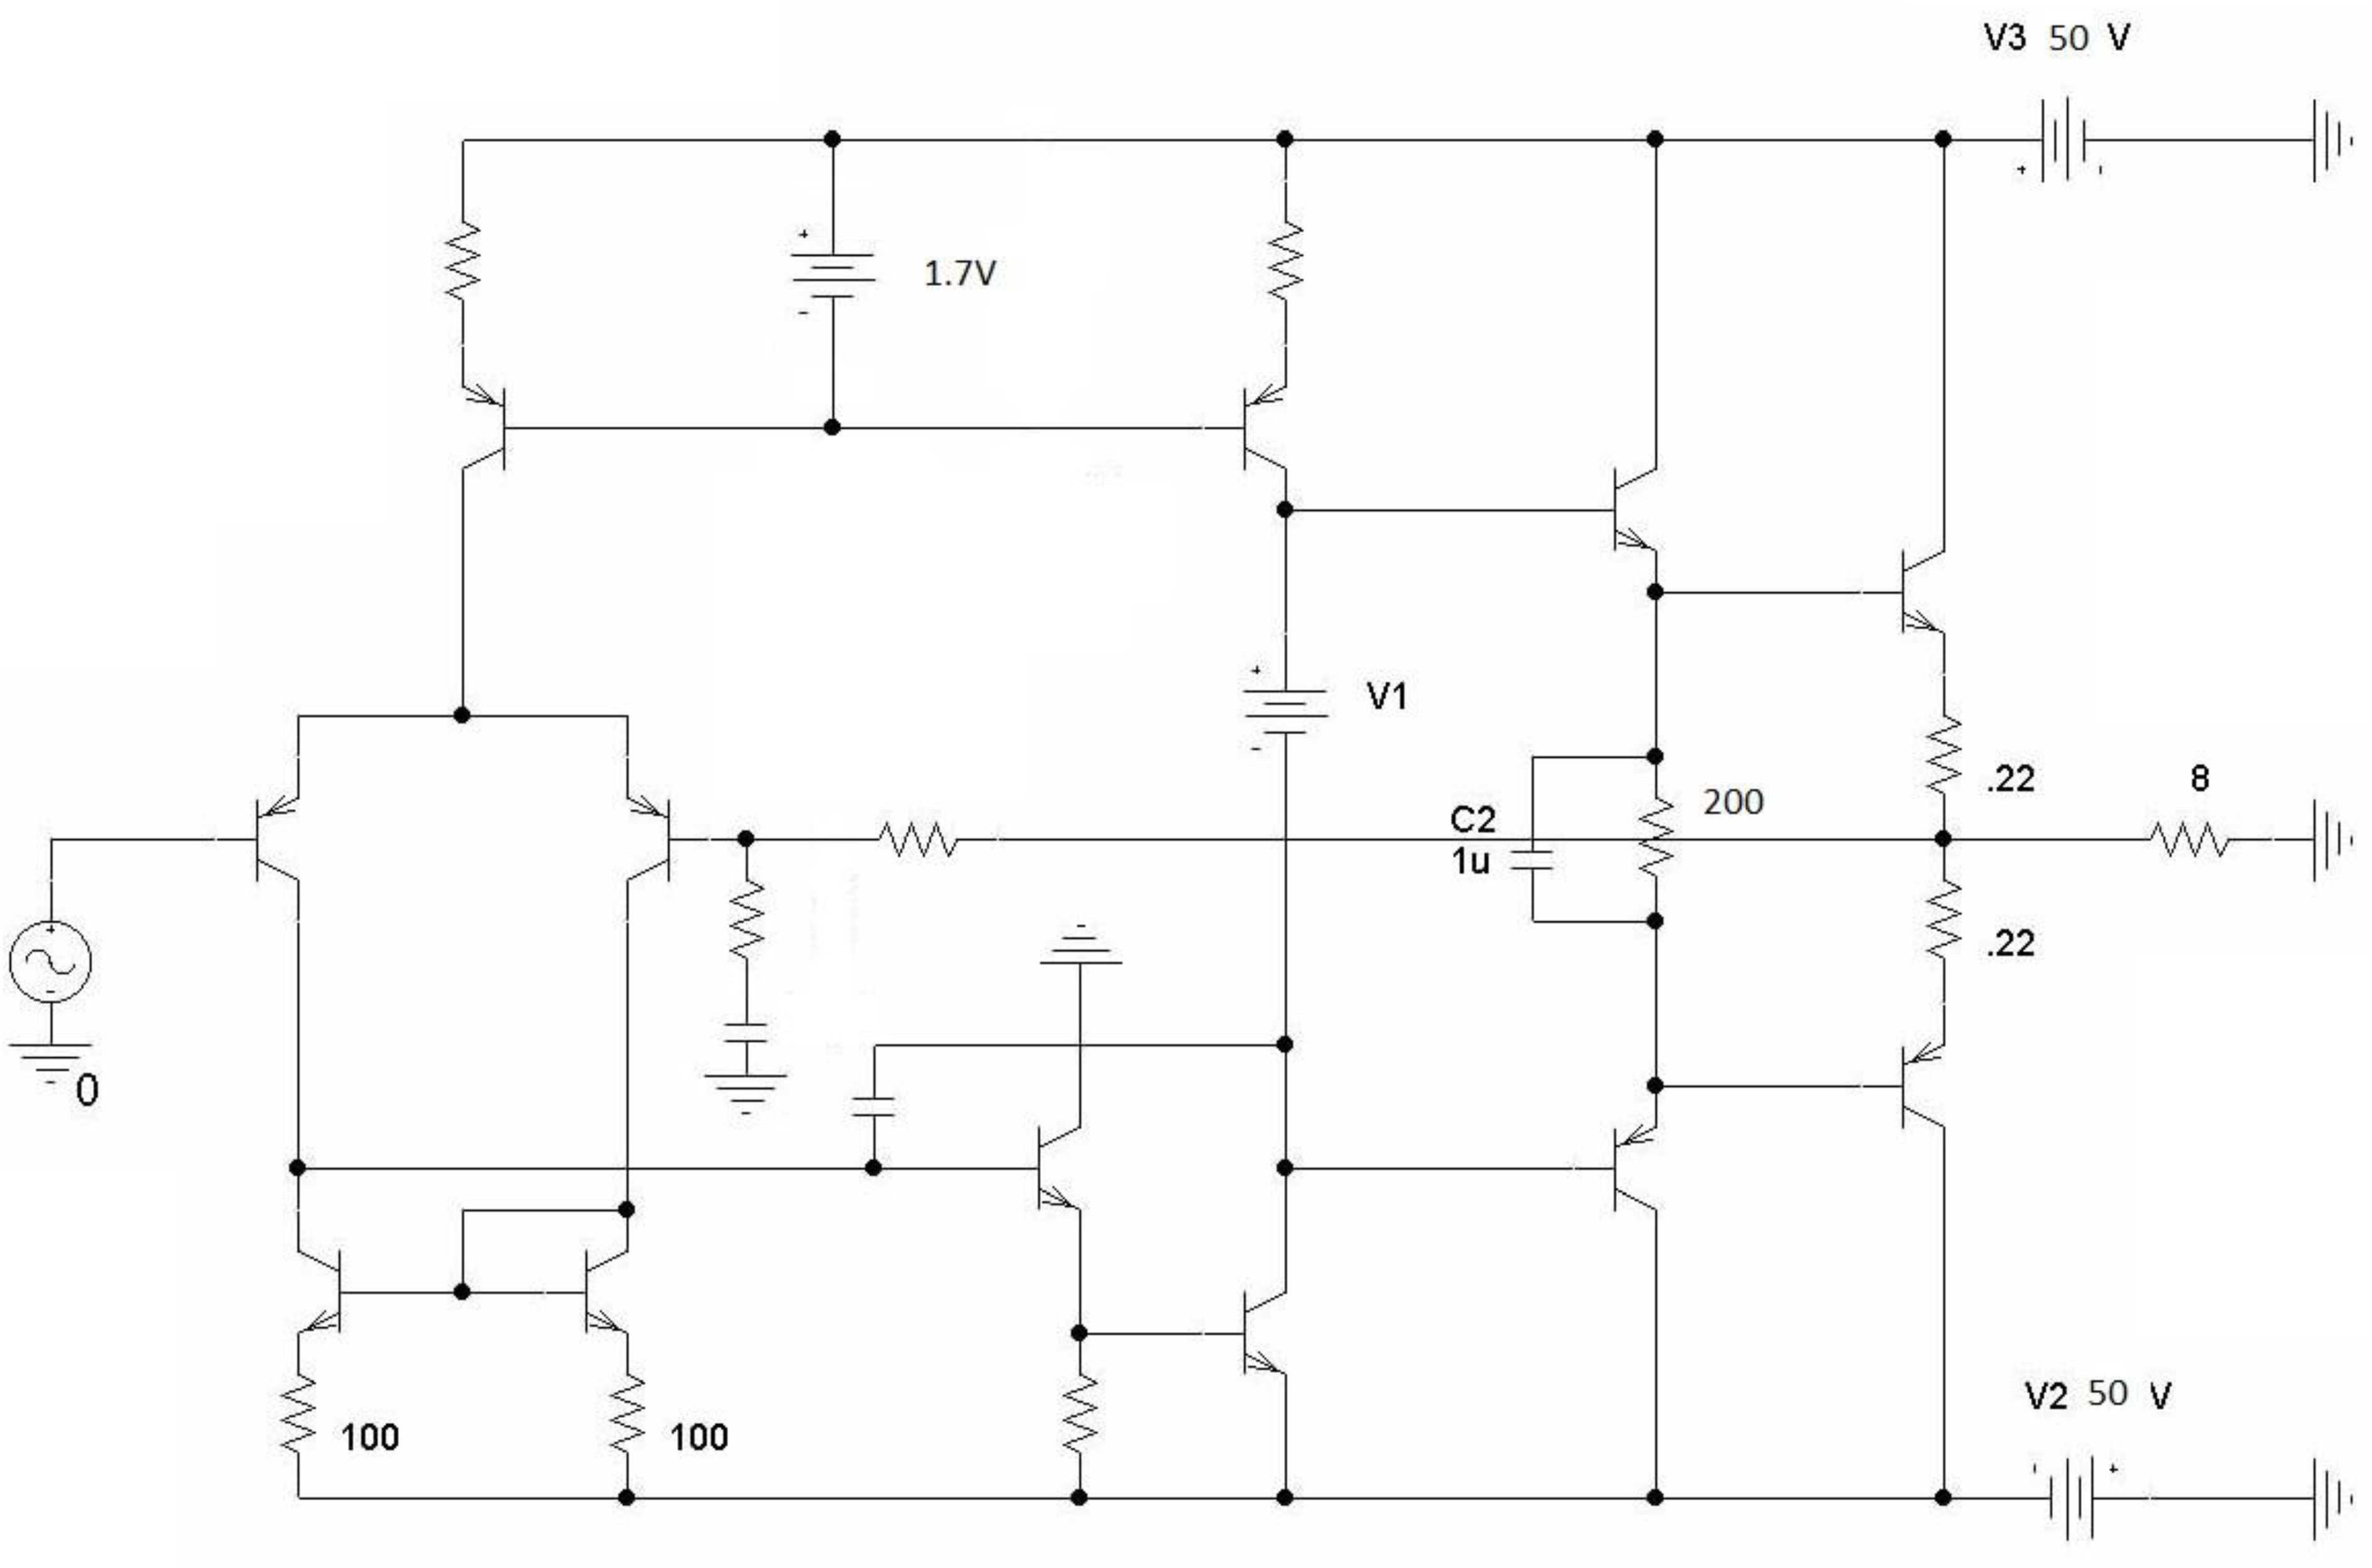
\includegraphics[width=1.0 \textwidth, angle=0]{./img/enunciado/circuito_enunciado.png}
\caption{\label{fig:fig_original_circuit}\footnotesize{Circuito propuesto.}}
\end{center}
\end{figure}


\clearpage
